% shared-memory-model.tex

\documentclass{standalone}

\usepackage{tikz}
\usetikzlibrary{positioning, arrows.meta, backgrounds, fit}

\begin{document}
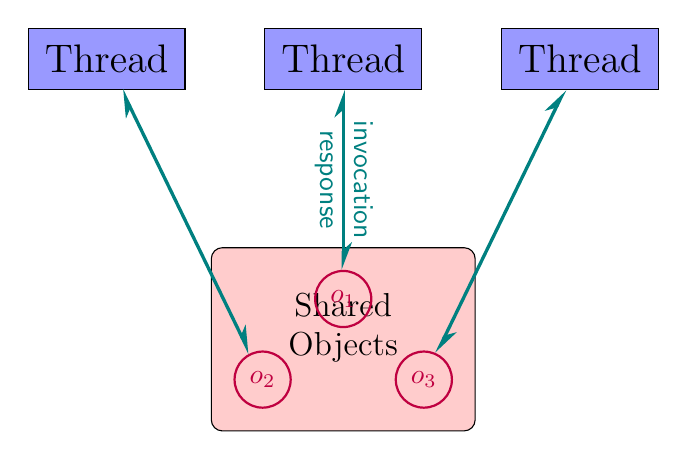
\begin{tikzpicture}[thread/.style = {draw, rectangle, fill = blue!40, font = \Large, inner sep = 6pt},
    call/.style = {{Stealth[left]}-{Stealth[left]}, very thick, teal},
    obj/.style = {draw, circle, thick, purple, minimum size = 5pt}]
  \node (o1) [obj] {$o_1$};
  \node (o2) [obj, below left = 0.50cm and 0.50cm of o1] {$o_2$};
  \node (o3) [obj, below right = 0.50cm and 0.50cm of o1] {$o_3$};
  \begin{pgfonlayer}{background}
    \node (so) [draw, rectangle, rounded corners, fit = (o1) (o2) (o3),
	  font = \large, fill = red!20, align = center, inner sep = 8pt] {Shared \\ Objects};
  \end{pgfonlayer}

  \node (tm) [thread, above = 2.0cm of so] {Thread};
  \node (tl) [thread, left = of tm] {Thread};
  \node (tr) [thread, right = of tm] {Thread};

  \draw [call] (tm) to node [above, sloped] {\textsf{invocation}} 
  	node [below, sloped] {\textsf{response}} (o1);
  \draw [call] (tl) to (o2);
  \draw [call] (tr) to (o3);
\end{tikzpicture}
\end{document}